\subsection{Game of Life Results}
\label{golres}
\subsubsection{NOT-gate}
\begin{figure}[H]
  \centering
  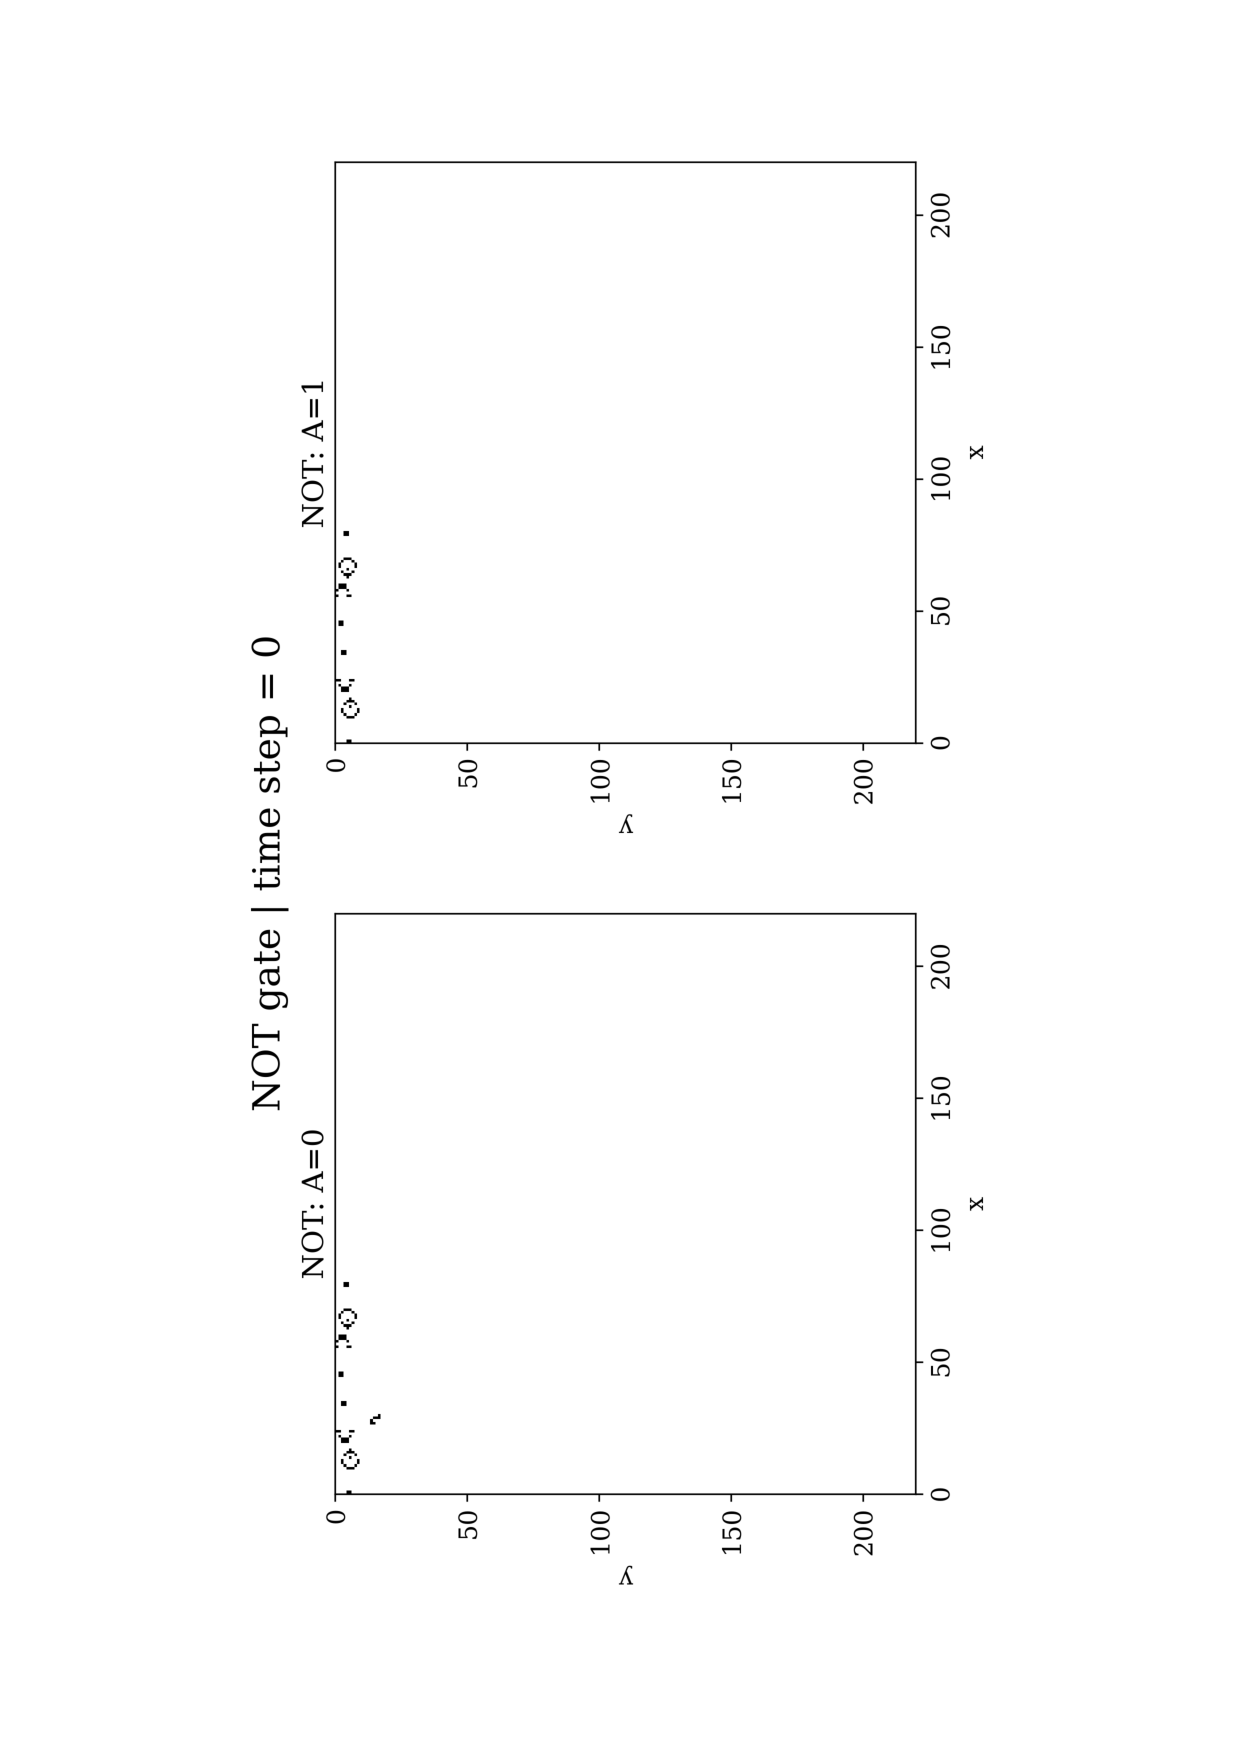
\includegraphics[width=\textwidth]{figs/GoL/NOT_t0.pdf}
  \caption{what happens here?}
  \label{fig:NOT_0}
\end{figure}
\begin{figure}[H]
  \centering
  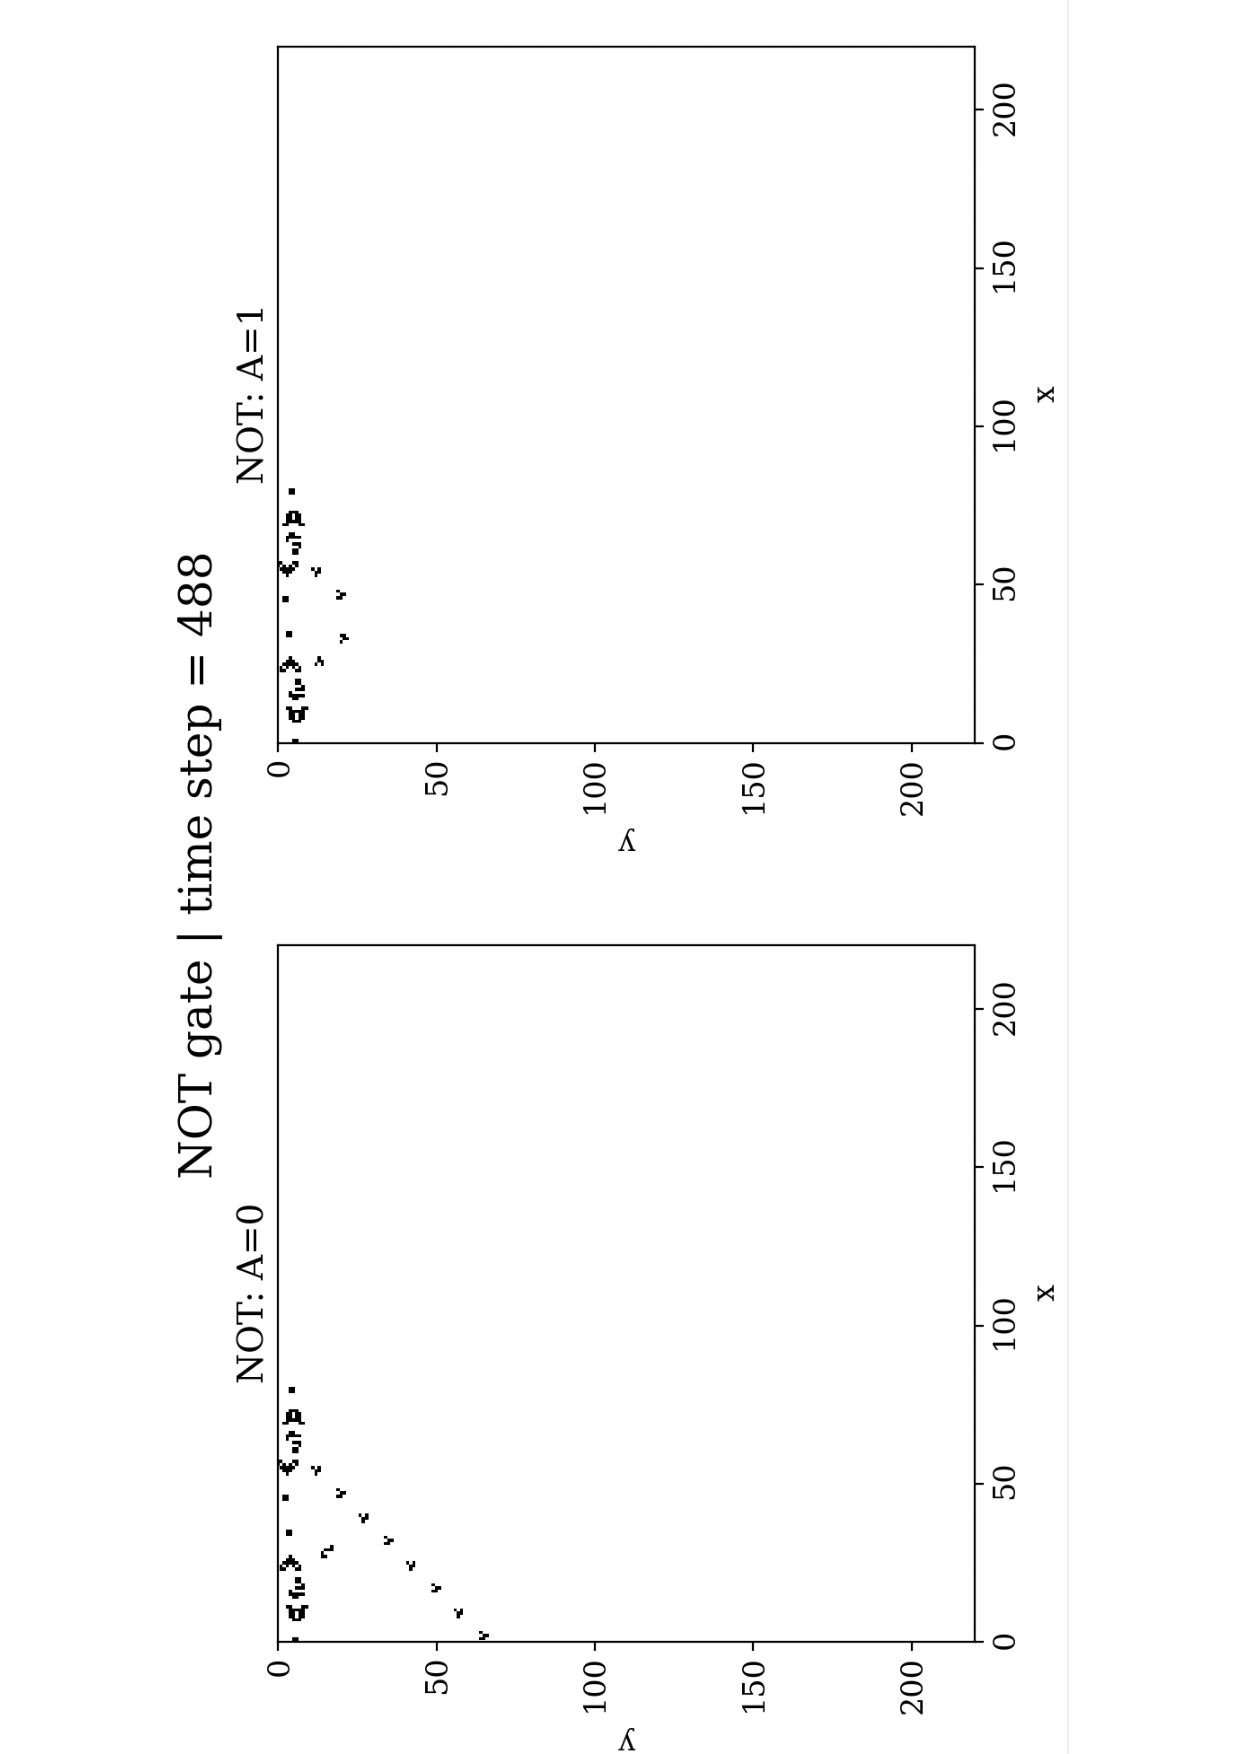
\includegraphics[width=\textwidth]{figs/GoL/NOT_Gate.pdf}
  \caption{what happens here?}
  \label{fig:NOT}
\end{figure}

For the NOT gate, there is only one input channel, $A$. The input glider moves diagonally from the top to the lower-right part of the grid. The output is observed after the interaction region, in the outgoing diagonal channel. The construction is arranged so that when $A=0$ an output glider survives, while when $A=1$ the input glider destroys or blocks the outgoing signal. Therefore, the NOT gate produces the opposite value of the input.

\subsubsection{AND-gate}
\begin{figure}[H]
  \centering
  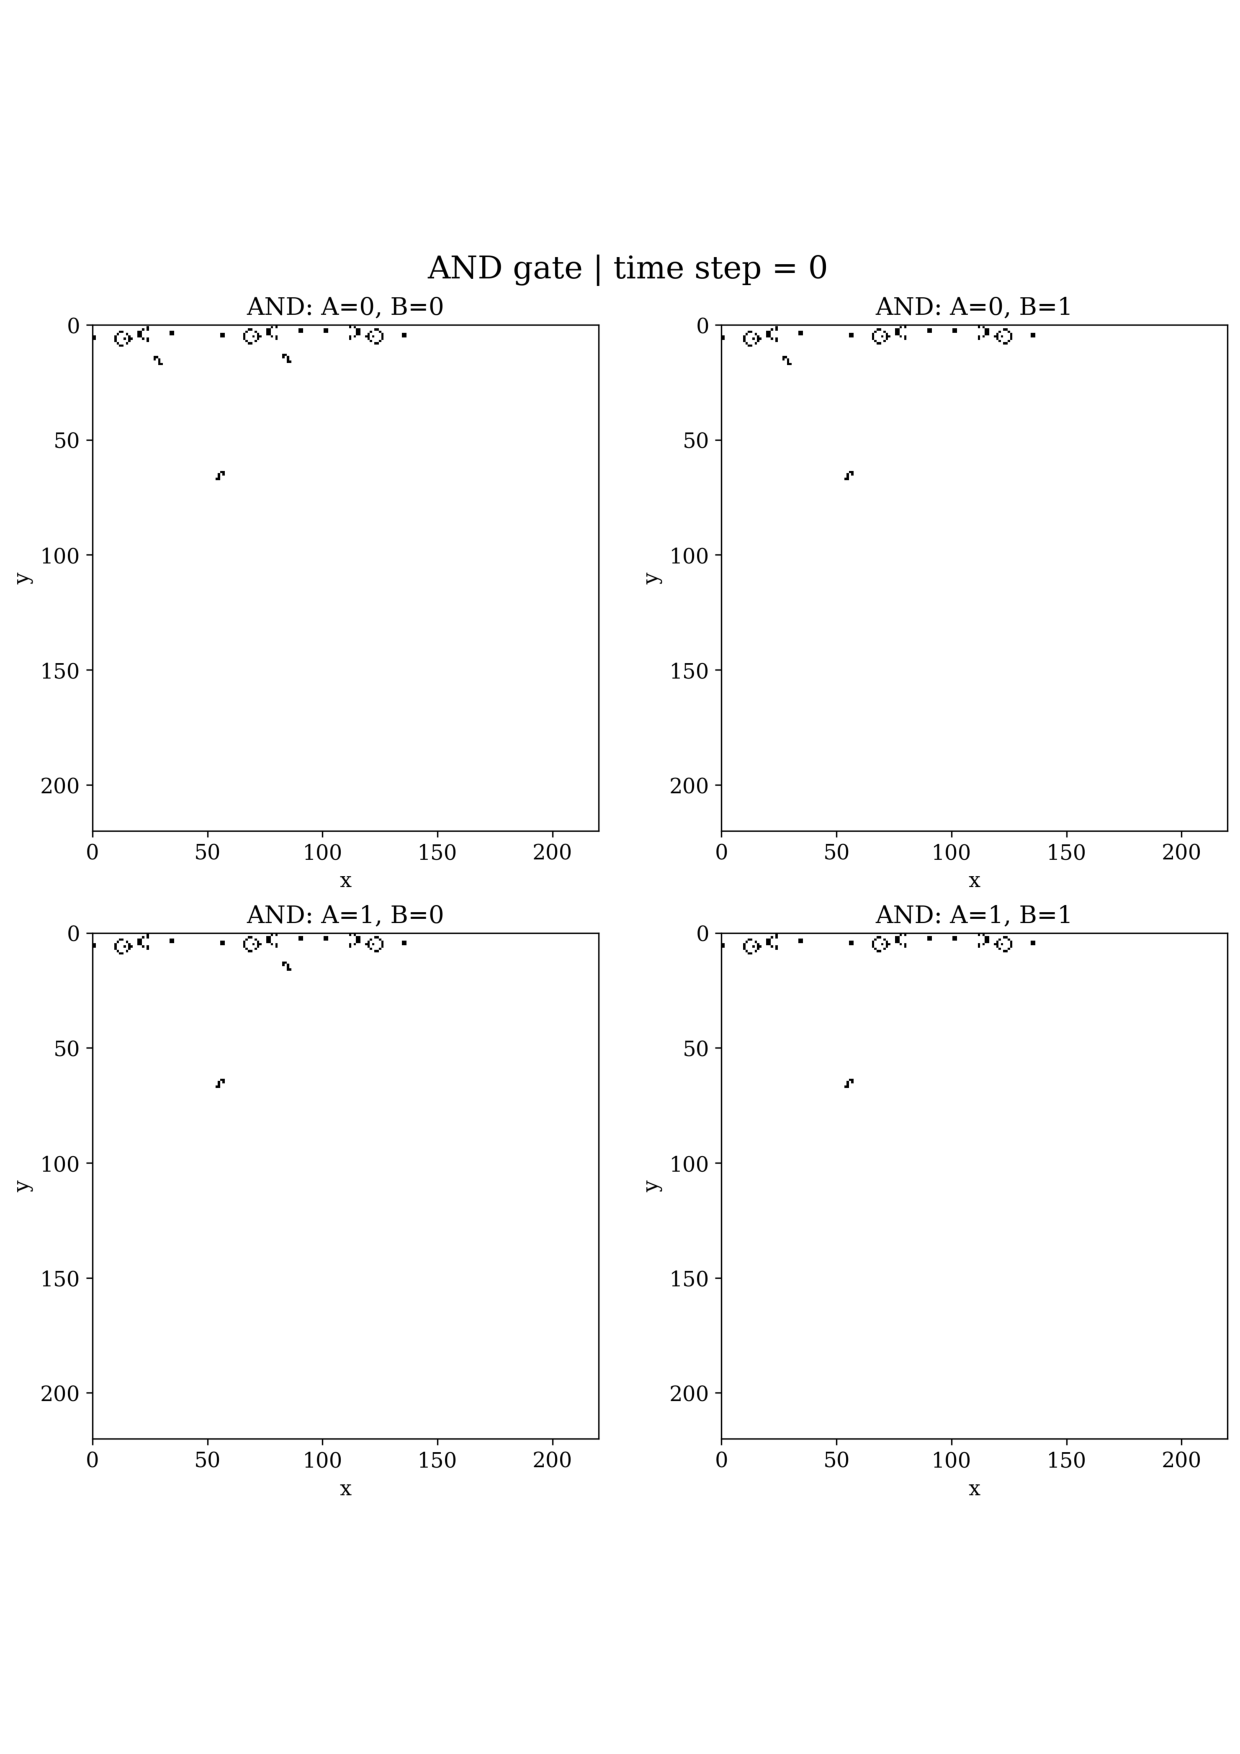
\includegraphics[width=\textwidth]{figs/GoL/AND_t0.pdf}
  \caption{what happens here?}
  \label{fig:AND_0}
\end{figure}
\begin{figure}[H]
  \centering
  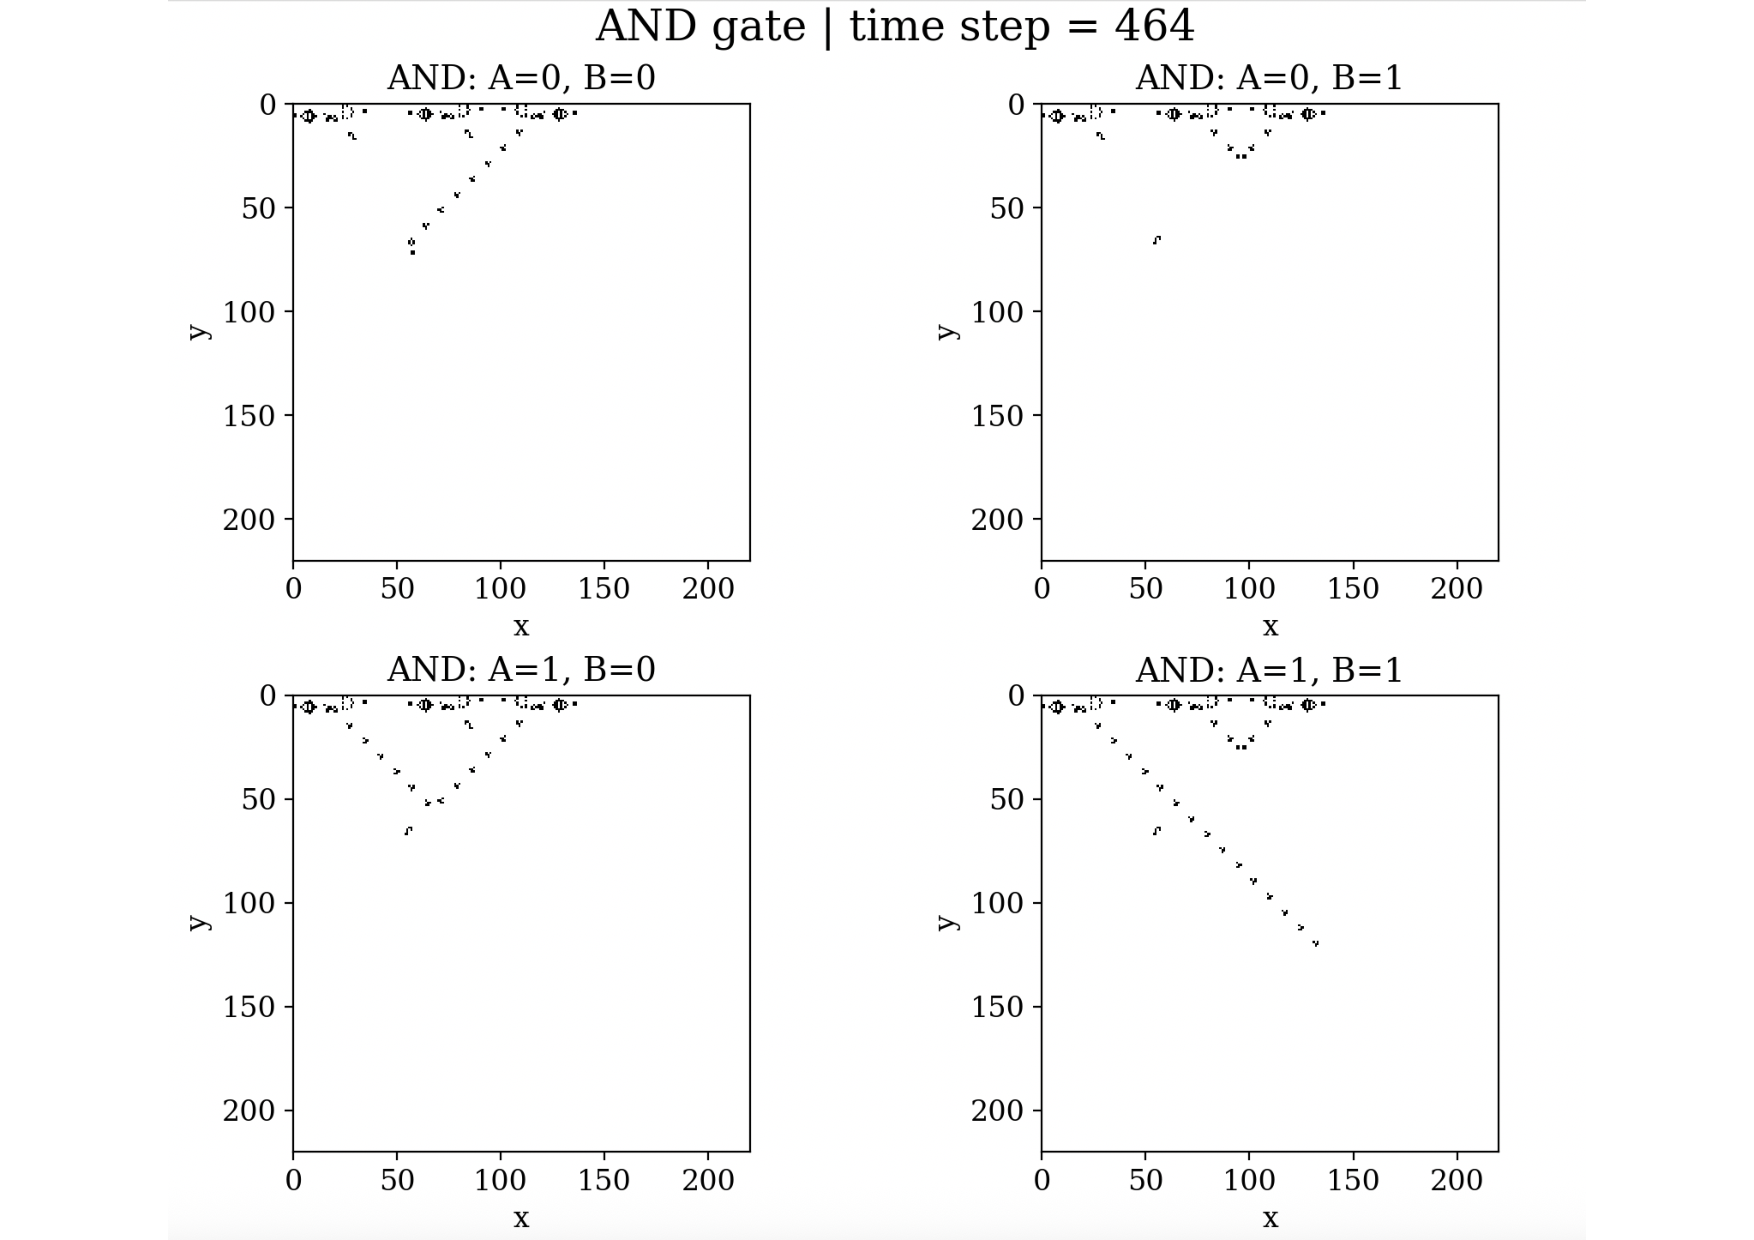
\includegraphics[width=\textwidth]{figs/GoL/AND_Gate.pdf}
  \caption{what happens here?}
  \label{fig:AND}


For the AND gate, two input channels are used, $A$ and $B$. The input gliders move diagonally from the top of the grid towards the lower-right part of the grid, where they interact with the gate structure. The output is observed in the outgoing diagonal channel after this interaction. A glider appears in the output channel only when both input gliders are present, so the output is $1$ only for $A=1$ and $B=1$.

\end{figure}
\subsubsection{OR-gate}
\begin{figure}[H]
  \centering
  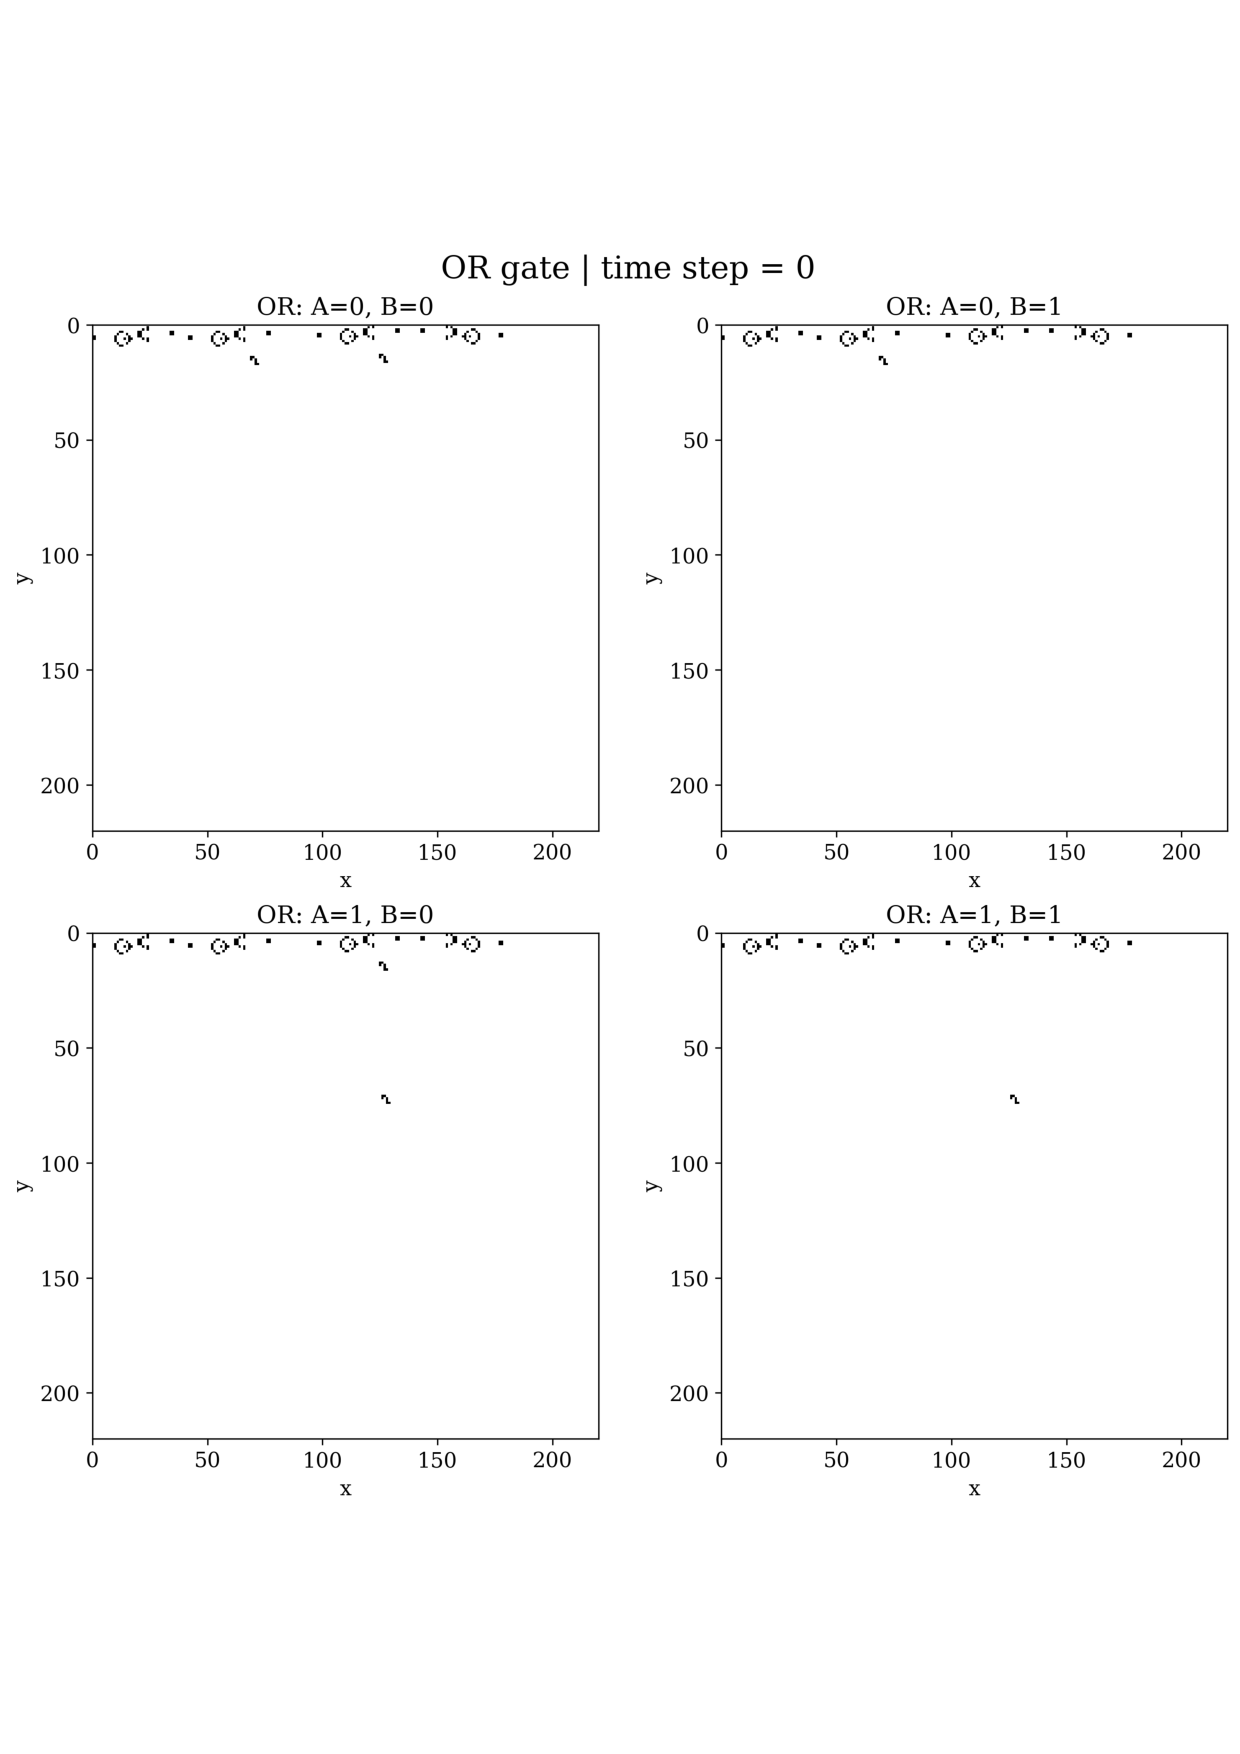
\includegraphics[width=\textwidth]{figs/GoL/OR_t0.pdf}
  \caption{what happens here?}
  \label{fig:OR_t0}
\end{figure}
\begin{figure}[H]
  \centering
  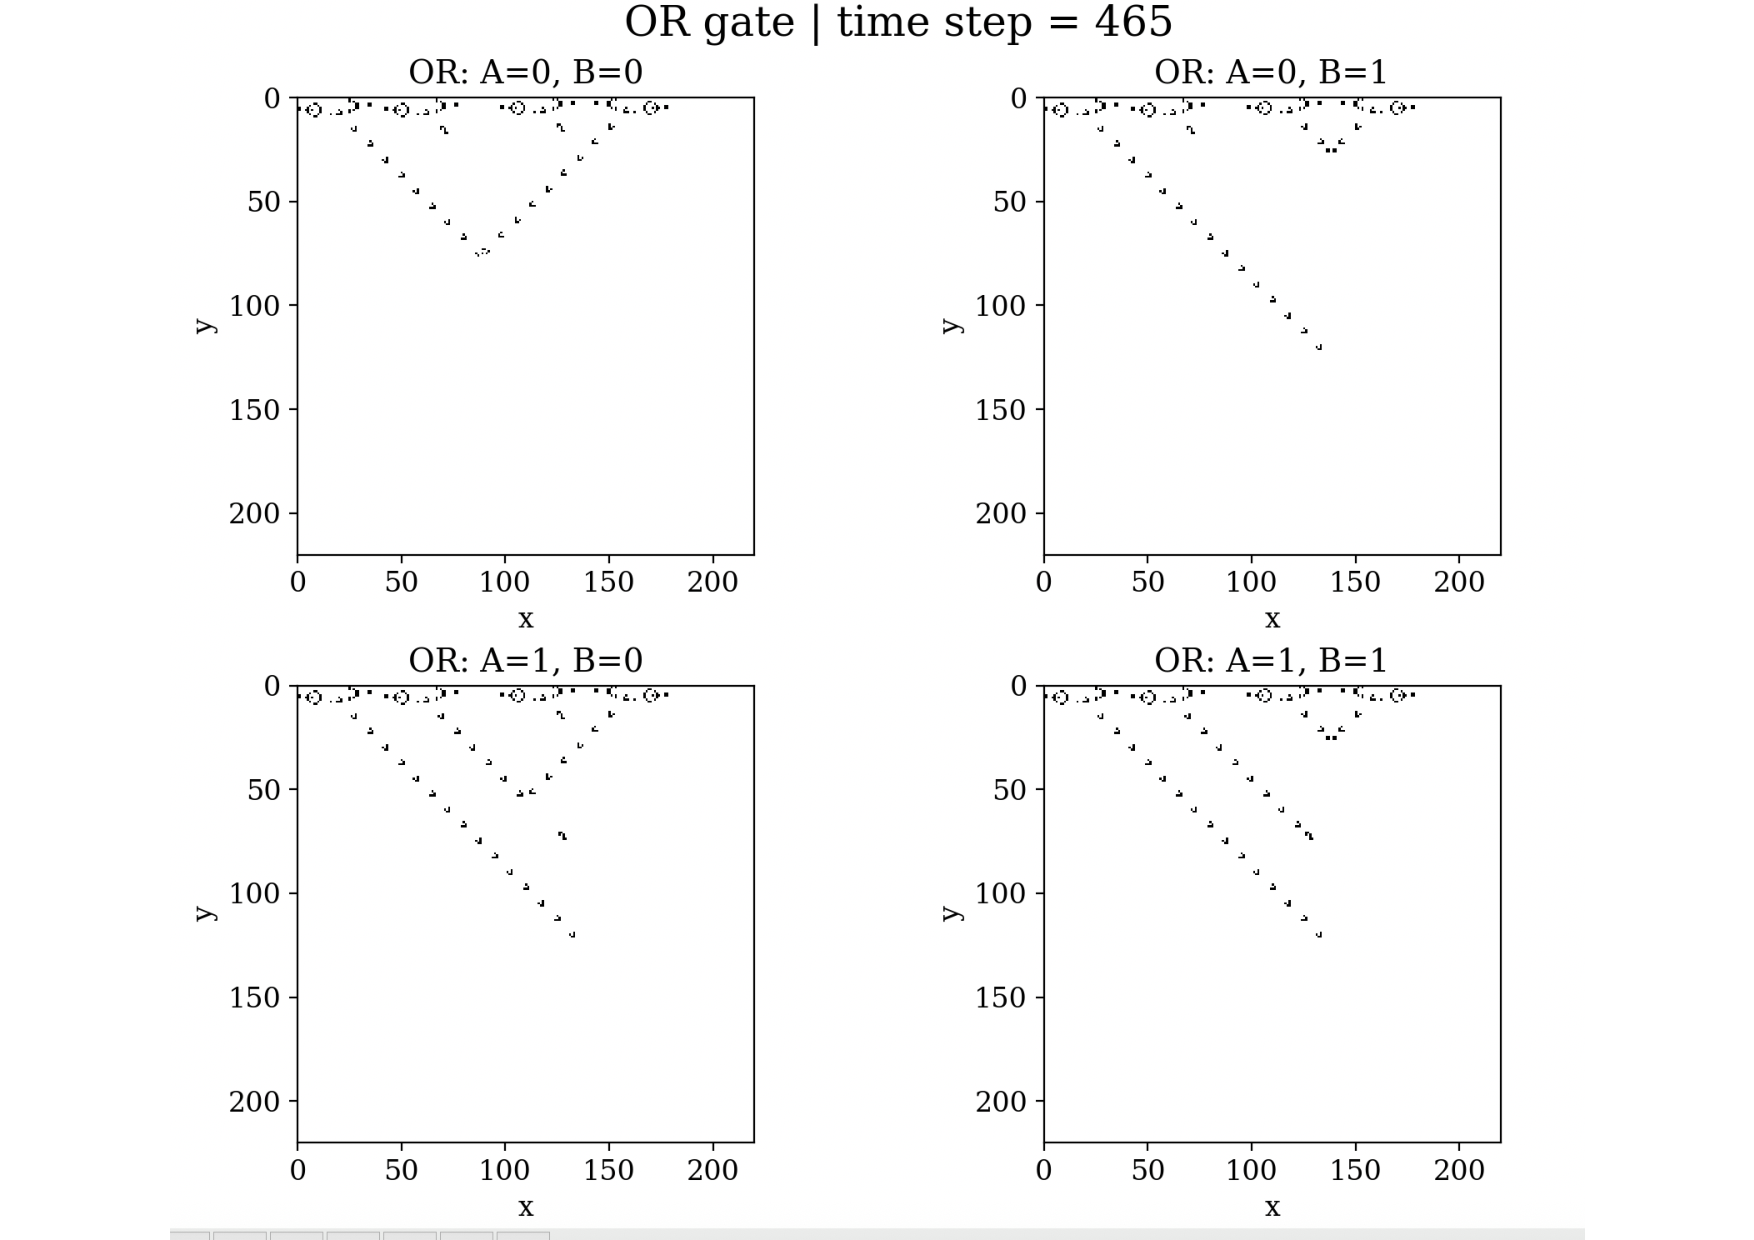
\includegraphics[width=\textwidth]{figs/GoL/OR_Gate.pdf}
  \caption{what happens here?}
  \label{fig:OR}
\end{figure}

For the OR gate, the input gliders also move diagonally from the top of the grid towards the lower-right part of the grid. The output is shown in the outgoing diagonal channel after the region of collision. In this case, the output channel contains a glider when, at least, one of the two input gliders is present.

\paragraph{Input and output directions in the Game of Life gates.}




